\documentclass[11pt,a4paper,titlepage]{article}
\usepackage[utf8]{inputenc}
\usepackage[english,polish]{babel}
\usepackage[T1]{fontenc}
\usepackage{polski}
\usepackage[math,light]{anttor}
\usepackage{amsmath}
\usepackage{amsfonts}
%\usepackage{amssymb}
\usepackage{graphicx}
\usepackage{sidecap}
%\usepackage{wrapfig}
\usepackage{epstopdf}
\usepackage{booktabs}
\usepackage{forloop}
\usepackage[left=3cm,right=3cm,top=3cm,bottom=3cm]{geometry}
\usepackage[framed,numbered,autolinebreaks]{mcode}
\usepackage[colorlinks=false,hidelinks,urlcolor=blue,citecolor=green]{hyperref}
\usepackage{fancyhdr}
\usepackage{lastpage}
\usepackage{array}
\usepackage{hhline}
\usepackage{multirow}
\usepackage {float}
\usepackage{enumerate}%[I], numerki, [(a)]
%ustawienie poziomów wypunktowania do wyboru: $\bullet$, $\cdot$, $\diamond$, $-$, $\ast$ and $\circ$ 
\renewcommand{\labelitemi}{$\diamond$}
\renewcommand{\labelitemii}{$\bullet$}
\renewcommand{\labelitemiii}{$-$}
\renewcommand{\labelitemiv}{$\ast$}


\AtBeginDocument{

	\renewcommand{\tablename}{Tabela}

	\renewcommand{\figurename}{Rys.}
}

%tabelki
\usepackage{tabularx}
\newcolumntype{A}{>{\centering\arraybackslash}X}
\newcolumntype{B}{>{\centering\arraybackslash} m{0.4\textwidth} }




\usepackage{csquotes}
\DeclareQuoteAlias{croatian}{polish} % Ponieważ `csquotes` nie posiada polskiego stylu, można skorzystać z mocno zbliżonego stylu chorwackiego.

%\addbibresource{bibliografia.bib}

\pagestyle{fancy}
\fancyhf{}
\fancyhead[R]{\slshape{\small \rightmark}}
\fancyfoot[R]{Wahadło odwrócone}
\fancyhead[L]{M. Cebula, P. Merynda, M. Podsiadło}     
\fancyfoot[L]{Strona \thepage \hspace{1pt} z\hspace{1pt} \pageref*{LastPage}}    
\renewcommand{\headrulewidth}{1pt}
\renewcommand{\footrulewidth}{1pt}


\begin{document}

\begin{titlepage}

\newcommand{\HRule}{\rule{\linewidth}{0.5mm}} % Defines a new command for the horizontal lines, change thickness here

\center % Center everything on the page
 
%----------------------------------------------------------------------------------------
%	HEADING SECTIONS
%----------------------------------------------------------------------------------------

\textsc{\LARGE Akademia Górniczo - Hutnicza im. Stanisława Staszica}\\[0.5cm]

\includegraphics[scale=0.6]{agh}\\[1cm] % Name of your university/college
\textsc{\Large Wydział Elektrotechniki, Automatyki, Informatyki i Inżynierii Biomedycznej}\\[0.5cm] % Major heading such as course name
\textsc{\large Katedra Automatyki i Inżynierii Biomedycznej}\\[0.5cm]
\textsc{ Kierunek: Automatyka i robotyka}\\[0.5cm] % Minor heading such as course title

%----------------------------------------------------------------------------------------
%	TITLE SECTION
%----------------------------------------------------------------------------------------

\HRule \\[0.4cm]
{ \huge \bfseries Procesory Sygnałowe i Mikrokontrolery\\[1cm]Generator sygnału wzorcowego na podstawie zadanej charakterystyki częstotliwościowej}\\[0.4cm] % Title of your document
\HRule \\[1.0cm]
 


%----------------------------------------------------------------------------------------
%	DATE SECTION
%----------------------------------------------------------------------------------------

%{\large \today}\\[1.5cm] % Date, change the \today to a set date if you want to be precise

%----------------------------------------------------------------------------------------
%	LOGO SECTION
%----------------------------------------------------------------------------------------

%
\includegraphics[height=70mm]{agh.jpg}%\\[1cm] % Include a department/university logo - this will require the graphicx package
%----------------------------------------------------------------------------------------
%	AUTHOR SECTION
%----------------------------------------------------------------------------------------

\begin{flushleft}
\Large
\emph{Wykonali:}\\
Maciej Cebula\\
Piotr Merynda\\
Maciej Podsiadło\\[1cm]

% If you don't want a supervisor, uncomment the two lines below and remove the section above
 \emph{Prowadzący:}\\
dr inż. Tomasz Dziwiński\\[3cm] % Your name
 
\end{flushleft}
%----------------------------------------------------------------------------------------
\end{titlepage}
\clearpage
\setcounter{page}{2}

\section{Wstęp}
Celem projektu było stworzenie generatora sygnału wzorcowego na podstawie zadanej charakterystyki częstotliwościowej. Do realizacji zadania postanowiono skorzystać ze sprzętu laboratoryjnego, na który składały się:
\begin{enumerate}
\item Komputer klasy PC,
\item Zestaw startowy z mikrokontrolerem z rodziny STM32 (STM32F401),
\item Oscyloskop.
\end{enumerate}
Korzystano z oprogramowania znajdującego się na PC, na którym zainstalowany jest system operacyjny Windows, a w szczególności z:
\begin{enumerate}
\item STM32CubeMX - graficznego środowiska umożliwiającego szybką konfigurację układów peryferialnych wraz generację szablonu kodu w języku C,
\item SW4STM32 - środowiska umożliwiającego szybkie tworzenie oraz debugowanie napisanego kodu,
\item MATLAB - zintegrowanego środowiska programistycznego, w którym stworzono prototyp algorytmu oraz interfejs u użytkownika.
\end{enumerate}
Zdecydowano, że docelowo użytkownik zadawał będzie punkty charakterystyki z poziomu aplikacji napisanej w MATLABie. Informacje te przesłane zostaną do mikrokontrolera poprzez interfejs szeregowy zgodnie ze standardem RS-232. Mikrokontroler wygeneruje odpowiedni sygnał wzorcowy, a następnie wyśle go do przetwornika cyfrowo-analogowego. Sygnał wyjściowy możliwy będzie do obejrzenia na oscyloskopie.





\section{Konfiguracja}
\subsection{Konfiguracja timerów}

\subsection{Konfiguracja przetwornika DAC}

\subsection{Konfiguracja portu szeregowego}

Do przesyłania danych z komputera do mikrokontrolera wykorzystany został protokół szeregowy \textit{RS232}. Parametry charakteryzujące transmisję podane są w tabeli \ref{tab_rs232}.

\begin{table}[h]
	\caption{Parametry portu szeregowego.}
	\label{tab_rs232}
	\centering
	
	\begin{tabular}{|c|c|}
		\hline
		\textbf{Parametr} & \textbf{Wartość}\\
		\hline
		Prędkość transmisji & 115200 Bitów/s \\
		\hline
		Długość słowa & 8 bitów \\
		\hline
		Bit parzystości & - \\
		\hline
		Bit stopu & 1 \\
		\hline
	\end{tabular}
\end{table}   
\section{Algorytm}
\subsection{Dyskretna transformacja Fouriera}
Głównym narzędziem matematycznym, które wykorzystano do rozwiązania postawionego zadania była odwrotna transformacja Fouriera. Przesłana przez użytkownika charakterystyka częstotliwościowa reprezentowana będzie poprzez wektor próbek. Dodatkowo biorąc pod uwagę fizyczne ograniczenia, w tym niezerowy czas działania przetwornika postanowiono wykorzystać algorytm odwrotnej dyskretnej transformacji Fouriera (IDFT). 

Oznaczając prze $N$ liczbę punktów charakterystyki częstotliwościowej zadanych przez użytkownika wprowadzono następujące oznaczenia:
\begin{align*} 
&freq = [f_1, f_2, ..., f_N]^T \\ 
&amp = [A_1, A_2, ..., A_N]^T \\
&phase = [\phi_1, \phi_2, ..., \phi_N]^T
\end{align*}
gdzie $freq$ jest wektorem niezerowych częstotliwości składowych zadanego sygnału, natomiast $amp$ oraz $phase$ odpowiadających im amplitud i przesunięć fazowych. Taki zabieg pozwala na zwarty zapis formuły:
\begin{equation}
x(k\Delta t) = \sum_{n=1}^{N}A_n\cdot\cos(2 \pi f_nk \Delta t - \phi_n), \quad k=0,1,2,...
\end{equation}
umożliwiającej wyliczenie kolejnych wartości sygnału spróbkowanego z częstotliwością $f_p=\frac{1}{\Delta t}$, którego charakterystyka częstotliwościowa została zadana.

\subsection{Prototyp algorytmu}



\section{Implementacja}
\subsection{Interfejs użytkownika}

\subsection{Protokół komunikacyjny}

\subsection{Generacja sygnału wyjściowego}
\section{Wnioski}
\indent W celu analizy porównawczej sygnałów uzyskanych na wyjściu z przetwornika DAC oraz sygnałów wzorcowych wygenerowanych w środowisku Matlab zapisano przesłane na oscyloskopie przebiegi czasowe w formacie danych *.CSV. Następnie importując je do środowiska Matlab możliwe było przeskalowanie wcześniej wygenerowanych przebiegów wzorcowych. Po przeskalowaniu i dopasowaniu fazy możliwe było zestawienie na jednym wykresie syganłów zadanych oraz sygnałów wygenerowanych przez układ. Wyniki kilku eksperymentów przedstawione są na rysunkach \ref{fig:10_100}, \ref{fig:10_100_1000} i \ref{fig:50_60}, gdzie kolorem niebieskim zaznaczony jest przebieg wygenerowany przez układ, natomiast kolorem czerwonym przebieg wzorcowy. Parametry podane jako wejście do układu zestawione zostały w tabelach \ref{tab_10_100}, \ref{tab_10_100_1000} i \ref{tab_50_60}.

\begin{table}[h]
	\caption{Parametry pierwszego przebiegu.}
	\label{tab_10_100}
	\centering
	
	\begin{tabular}{|c|c|c|}
		\hline
		\textbf{Częstotliwość [Hz]} & \textbf{Amplituda} & \textbf{Przesunięcie fazowe [\textdegree]}\\
		\hline
		10 & 7 & 180 \\
		\hline
		100 & 2 & 0 \\
		\hline
	\end{tabular}
\end{table}

\begin{figure}[h!]
	\centering
	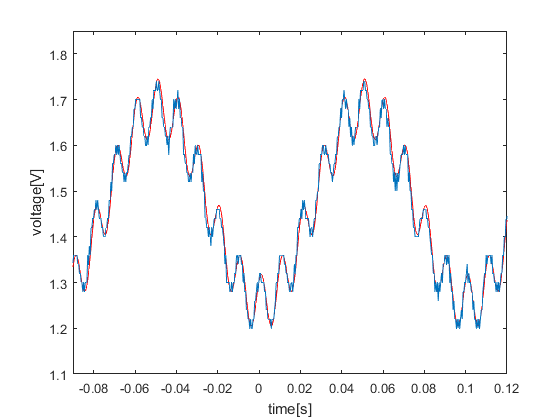
\includegraphics[scale = 0.8]{fig/10_100.png}
	\caption		
	{Zestawienie przebiegu wygenerowanego przez układ z przebiegiem wzorcowym dla parametrów z tabeli \ref{tab_10_100}.}
	\label{fig:10_100}
\end{figure}

\begin{table}[h]
	\caption{Parametry drugiego przebiegu.}
	\label{tab_10_100_1000}
	\centering
	
	\begin{tabular}{|c|c|c|}
		\hline
		\textbf{Częstotliwość [Hz]} & \textbf{Amplituda} & \textbf{Przesunięcie fazowe [\textdegree]}\\
		\hline
		10 & 7 & 180 \\
		\hline
		100 & 2 & 0 \\
		\hline
		1000 & 2 & 0 \\
		\hline
	\end{tabular}
\end{table}

\begin{figure}[h!]
	\centering
	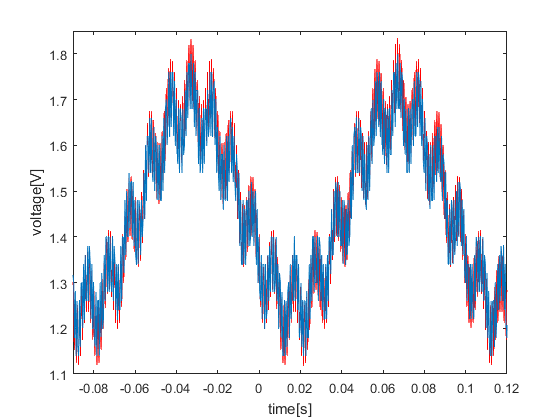
\includegraphics[scale = 0.8]{fig/10_100_1000.png}
	\caption		
	{Zestawienie przebiegu wygenerowanego przez układ z przebiegiem wzorcowym dla parametrów z tabeli \ref{tab_10_100_1000}}
	\label{fig:10_100_1000}
\end{figure}

\begin{table}[h]
	\caption{Parametry trzeciego przebiegu.}
	\label{tab_50_60}
	\centering
	
	\begin{tabular}{|c|c|c|}
		\hline
		\textbf{Częstotliwość [Hz]} & \textbf{Amplituda} & \textbf{Przesunięcie fazowe [\textdegree]}\\
		\hline
		50 & 4 & 180 \\
		\hline
		60 & 3 & 90 \\
		\hline
	\end{tabular}
\end{table}

\begin{figure}[H]
	\centering
	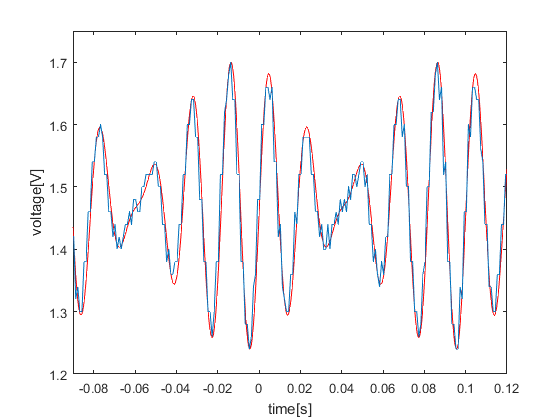
\includegraphics[scale = 0.8]{fig/50_60.png}
	\caption		
	{Zestawienie przebiegu wygenerowanego przez układ z przebiegiem wzorcowym dla parametrów z tabeli \ref{tab_50_60}}
	\label{fig:50_60}
\end{figure}

\indent Analizując przedstaione wyniki można zauważyć stosunkowo dobre dopasowanie wygenerowanych sygnałów do sygnałów wzorcowych. Widoczne na wykresie \ref{fig:50_60} ostre zmiany wartości wyjściowej tłumaczyć można jako niedokładność generowaną na zbliżeniu przez oscyloskop. Rozdzielczość, w której zapisane zostały serie danych wynosi 600x600 co generuje widoczne niedokładności.

\indent W ogólnym rozrachunku udało się zrealizowac wszystkie założenia projektowe. Realizację algorytmu genaracji sygnału na podstawie danych parametrów. Wysyłanie wyliczonych wartości na układ DAC. Interfejs użytkownika umożliwiający zadawanie parametrów sygnału oraz komunikację z mikrokontrolerem.

\newpage
\tableofcontents
\newpage
\nocite{*}
\end{document}